\documentclass[
a4paper, % Stock and paper size.
12pt, % Type size.
article,
% oneside,
onecolumn, % Only one column of text on a page.
% openright, % Each chapter will start on a recto page.
% openleft, % Each chapter will start on a verso page.
openany, % A chapter may start on either a recto or verso page.
]{memoir}
\synctex=1
\maxtocdepth{subsection}
\setsecnumdepth{subsection}
\counterwithout{section}{chapter}
%%% PACKAGES
%%%------------------------------------------------------------------------------
\usepackage[utf8]{inputenc} % If utf8 encoding
% \usepackage[lantin1]{inputenc} % If not utf8 encoding, then this is probably the way to go
\usepackage[T1]{fontenc}    %
\usepackage[russian,english]{babel} % English please


%%% Figures and colors
\usepackage[usenames,dvipsnames,svgnames,table,rgb]{xcolor}
\usepackage{tikz} % Figures. Following colors are predefined: red, green, blue, cyan, magenta, yellow, black, gray, darkgray, lightgray, brown, lime, olive, orange, pink, purple, teal, violet and white.

% Defining a new coordinate system for the page:
%
% --------------------------
% |(-1,1)    (0,1)    (1,1)|
% |                        |
% |(-1,0)    (0,0)    (1,0)|
% |                        |
% |(-1,-1)   (0,-1)  (1,-1)|
% --------------------------
\makeatletter
\def\parsecomma#1,#2\endparsecomma{\def\page@x{#1}\def\page@y{#2}}
\tikzdeclarecoordinatesystem{page}{
    \parsecomma#1\endparsecomma
    \pgfpointanchor{current page}{north east}
    % Save the upper right corner
    \pgf@xc=\pgf@x%
    \pgf@yc=\pgf@y%
    % save the lower left corner
    \pgfpointanchor{current page}{south west}
    \pgf@xb=\pgf@x%
    \pgf@yb=\pgf@y%
    % Transform to the correct placement
    \pgfmathparse{(\pgf@xc-\pgf@xb)/2.*\page@x+(\pgf@xc+\pgf@xb)/2.}
    \expandafter\pgf@x\expandafter=\pgfmathresult pt
    \pgfmathparse{(\pgf@yc-\pgf@yb)/2.*\page@y+(\pgf@yc+\pgf@yb)/2.}
    \expandafter\pgf@y\expandafter=\pgfmathresult pt
}
\makeatother

\usepackage{graphicx}  % Include figures
\usepackage{wrapfig}
\graphicspath{{img/}{../img/}} 


%%% INTERNAL HYPERLINKS
%%%-------------------------------------------------------------------------------

\usepackage{hyperref}   % Internal hyperlinks
\newcommand{\linkcolor}{blue}
\newcommand{\citecolor}{blue}
\newcommand{\filecolor}{magenta}
\newcommand{\urlcolor}{NavyBlue}
\hypersetup{				% Гиперссылки
    pdfborder={0 0 0},      % No borders around internal hyperlinks
	unicode=true,           % русские буквы в раздела PDF\\
	pdfstartview=FitH,
	colorlinks=true,  % false: ссылки в рамках; true: цветные ссылки
	linkcolor=\linkcolor,         % внутренние ссылки
	citecolor=\citecolor,        % на библиографию
	filecolor=\filecolor,      % на файлы
	urlcolor=\urlcolor,      % на URL
    linkbordercolor=\linkcolor,  % hyperlink border will be red 
    pdftitle={Yoga Veera Kit},
    pdfpagemode=FullScreen,
    pdfauthor={I am the Author} % author
}

\let\oldhref\href
\renewcommand{\href}[2]{\oldhref{#1}{\underline{#2}}}


\graphicspath{{img/}{../img/}{../FreqImg/}}


%%% PAGE LAYOUT
%%%------------------------------------------------------------------------------

\setlrmarginsandblock{0.15\paperwidth}{*}{1} % Left and right margin
\setulmarginsandblock{0.10\paperwidth}{*}{1} % Upper and lower margin
\checkandfixthelayout
%%% indenting
\setlength{\parindent}{0em}
\setlength{\parskip}{0.5em}

\setsecnumdepth{subsection}
\maxtocdepth{subsection}



\begin{document}

\begin{center}
\Huge \textbf{Montage Guide RU}
\end{center}
\tableofcontents

\tikz[remember picture,overlay]
\node[opacity=0.9,inner sep=0pt] at (page cs:0.8,0.8)
{
\includegraphics[width=0.1\paperwidth]{IshaLogo}};

\subsection*{Preface}

Link to Google Drive with files for installation:
\href{https://ishaeu.org/RUMontage}{https://ishaeu.org/RUMontage}

We recommend reading the document directly on Google Drive (link
above), or a very recently downloaded version,
since the guide is periodically corrected and supplemented.


\newpage
\section{Recommendations for YouTube}\label{montageRules}
In the rules, we have identified the best practices that allow
us to maintain quality and maintain the overall style.

\subsection{Export Parameters}
\begin{itemize}
\item\textbf{format --- .mp4};
\item \textbf{codec --- H264};
\item \textbf{video bitrate~--- 10mbps};

If your Internet does not allow 10mbps, you can take the bitrate a little
higher than in the original video (usually somewhere 2-3 mbps).

\item \textbf{audio bitrate --- 320};
\item \textbf{resolution --- $1920 \times 1080$};

If the resolution of the original is $1280 \times 720$,
we make the original video in the format
$1920 \times 1080$ {\color{gray}(recommendation algorithms
YouTube is encouraged
high-format videos)}.

But, if it is $480$\ or lower --- then we leave
as the original {\color{gray}(stretch $480$ to $1080$
too much already)}.
\end{itemize}



\subsection{Splash screen at the end}

\begin{itemize}
\item The final slide should be replaced
with \href{https://drive.google.com/file/d/11NbSgvq8LbxDcy-a2WY5OJTKUZKcZx88/view?usp=sharing }{Russian}.

The final inscription <<\textcopyright\ Sadhguru 2021>> does not change.

Frequently used slides/music can be found on Google Drive in the folder
useful\_files.
\href{https://ishaeu.org/RUMontage}{https://ishaeu.org/RUMontage}
\end{itemize}


\subsection{Transitions}
\begin{itemize}
\item Transitions between fragments with different backgrounds via Dip to Black, otherwise via Dissolve.
\item Transitions for subtitles from texts are done through something like Cross Disolve.
\item Transitions should usually last about 1 sec.
More than 2 s, usually, --- overkill.
\end{itemize}

\subsection{Titles}
\begin{itemize}
\item There are two translations of titles in the task:
TN\_TITLE and TITLE.

\textbf{TN\_TITLE}~--- the text that will be on
thumbnail (screensaver on the video).

\textbf{TITLE}~--- the text title of the video.

Also, there will often be several variants of names
in TN\_TITLE and TITLE with one highlighted.

During installation, our
priority~--- TN\_TITLE, but you can choose any other
from the list. For example, if TN\_TITLE is too long,
or, for some reason, it will look bad.
\end{itemize}


\subsection{General requirements for the text}
\begin{itemize}
\item Ishi's design department gave the following fonts:
\textbf{Merriweather}~--- for headings and large text, and
\textbf{Open Sans}~--- for subtitles. We use them.

Sometimes \textbf{Segoe Script} is used, you will notice it immediately, an example is below.


\includegraphics[width=0.3\textwidth]{segoeScript}

They can be downloaded and installed from Google Fonts:
\begin{itemize}
\item Merriweather
\href{https://fonts.google.com/specimen/Merriweather}{\small https://fonts.google.com/specimen/Merriweather};
\item Open Sans
\href{https://fonts.google.com/specimen/Open+Sans}{\small https://fonts.google.com/specimen/Open+Sans};
\item Segoe Script
\href{https://www.fonts.com/font/microsoft-corporation/segoe-script?QueryFontType=Web&src=GoogleWebFonts}{\small https://www.fonts.com/font/microsoft-corporation/segoe-script?QueryFontType=Web\&src=GoogleWebFonts}.
\end{itemize}

\emph{P.S.} Installing fonts is very easy,
below (page \pageref{fonts}) you can find instructions for macOS.

\item Sometimes you have to insert text into the video.

\textbf{Ashram Recommendation}: Visual objects should not overlap
Sadhguru. If necessary~--- choose the lesser evil. We occupy the lower part,
completely leaving the face visible.

\item Any kind of complicated translation,
{\color{gray} if it has not already been provided with the task},
especially if there are some names, you need to coordinate
with the project coordinator.

\item Visual effects are selected according to the situation.
The most important thing is~--- to look neat. Variety and sophistication
effects ~--- in second place.

You can read more about the methods in the tips (page \pageref{advices}).

\textbf{Note}: usually, the text has an opaque background
it doesn't look like fire. When adding text over English,
if the background is not monochrome, it is usually better to add blur to English.
text, and on top of it ~--- translation with a translucent background.

\textbf{Note}: usually, when adding a subtitle with
background, it is better to round off the rectangular edges.
\end{itemize}



\subsection{Text translation}

\begin{itemize}

\item Inserts with text (for example, questions). If the text is not voiced,
the time of the fragment with the text should be sufficient so that you can
slowly read it (you may have to lengthen the video).

\item Sometimes in the English version, subtitles are inserted directly into the video
{\color{gray}(usually, during an unintelligible question)}. Should we translate them
\textbf{not} needed, because the Russian voice is clear,
and subtitles can always be turned on.

But, in the case when it's not subtitles, but a slide with a question ~---
you need to translate, even if the question is voiced.
\item The English text should not be visible during translation. For this, sometimes it is better
cover with a transfer with a margin of time on the left and right. That is, to cut
not exactly at the beginning and end, but with indents.

In the case of complex animation, this can be neglected for the sake of general aesthetics.


\item Titles about the place and date of the video recording, like "Darshan - Dec 2012
Isha Yoga Center" and similar non-essential text are left unchanged.

{\color{gray} Reasons: they are not worth the time spent, plus
subtitles with translation reduce the overall beauty.}

\item When a Sadhguru reads a poem and there is no Russian voiceover, when adding
more subtitles with Russian "free interpretation", it is better to break it into
several, each
by $\approx 3$ lines and add them at the bottom in the center.

\end{itemize}


\subsection{Old videos}

\begin{itemize}

\item For square videos, we duplicate it on the background, stretch it to the borders,
and apply blur.
\begin{center} 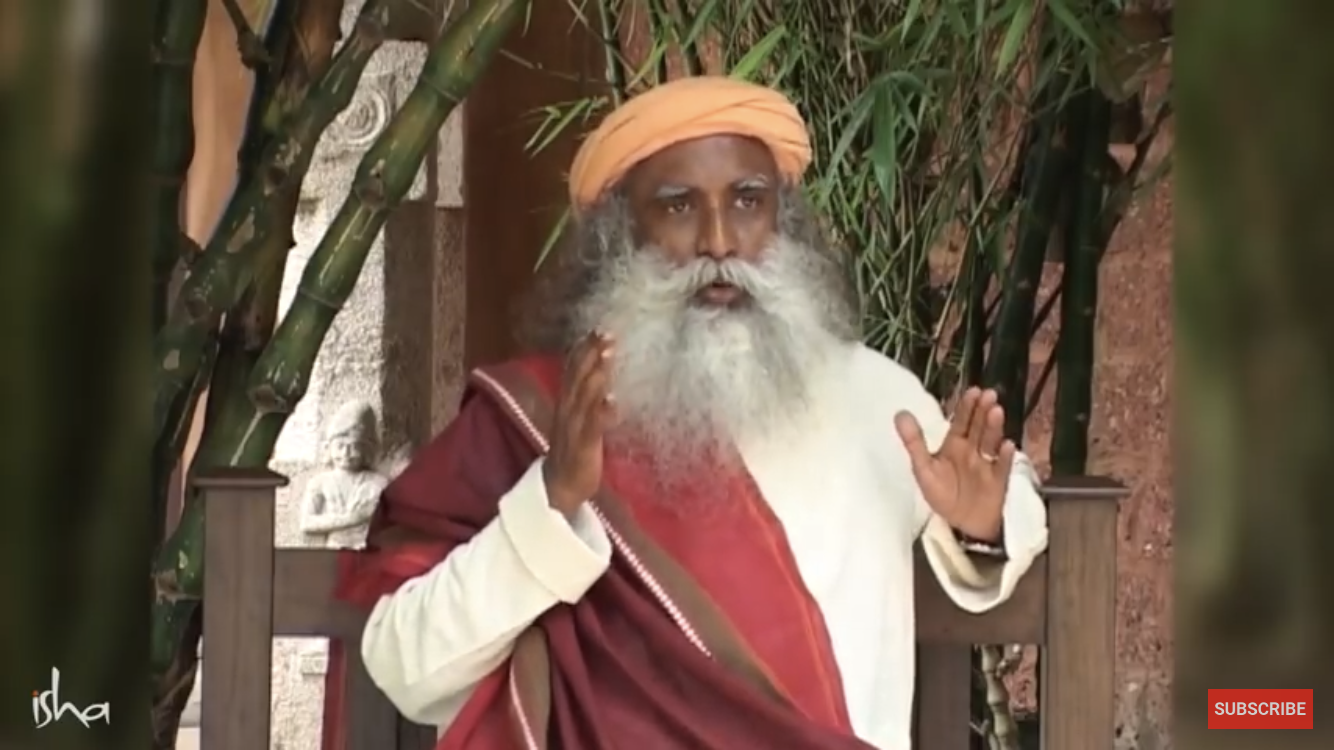
\includegraphics[width=0.5\textwidth]{tooWide} \end{center}

\item Outdated screensavers <<Sadhguru. Yogi, mystic and visioner.>> and
<<Conversation with Mystic>> are cut out.

{\color{gray}Reason: they are not particularly useful and take time.}
\end{itemize}


\subsection{Installation without audio}

\begin{itemize}
\item When an audio track is delayed, sometimes we mount it in two
stages: one volunteer mounts (almost) all the videos, and
the second~--- replaces the audio track.

In this case, the first editor of \textbf{should leave
the length of the video clip is unchanged}. That is, it is not worth cutting out
fragments or lengthen them.

Reason: it will usually be much easier for the second person
do it yourself (cut or lengthen), than then reduce the audio.
\end{itemize}

\newpage
\section{Tips}\label{advices}

\subsection{General tips}
\textbf{Be careful~--- and you won't have to redo it.}

Check that the text is gram-free. errors
that everything is in order with punctuation;
before installation, check in the modified fragments
that everything is neat;
after installation, also check these places.

The changed places are usually no more than 5, and it takes 2-3 minutes,
but it can save both your time for re-rendering
and the time of the inspector.

\textbf{Special attention}: check that you have not forgotten to mix the
English audio track.

\subsection{The main methods of text translation.}

\begin{itemize}
\item\emph{Overlay text with opaque background.}

\begin{itemize}
\item is suitable for a situation where the background in the place where the text
is placed is monochrome, but usually this is not the case, and it is better to use other methods.
\end{itemize}

\item \emph{Apply gaussian blur to the place where the text is located, and add
its on top.}

\begin{itemize}
\item Universal way, suitable for
dynamic background, and usually looks good.

\item Below is an example where it was better to use blur.

\begin{figure}[!hbp]
\centering
\begin{minipage}[b]{0.4\textwidth}
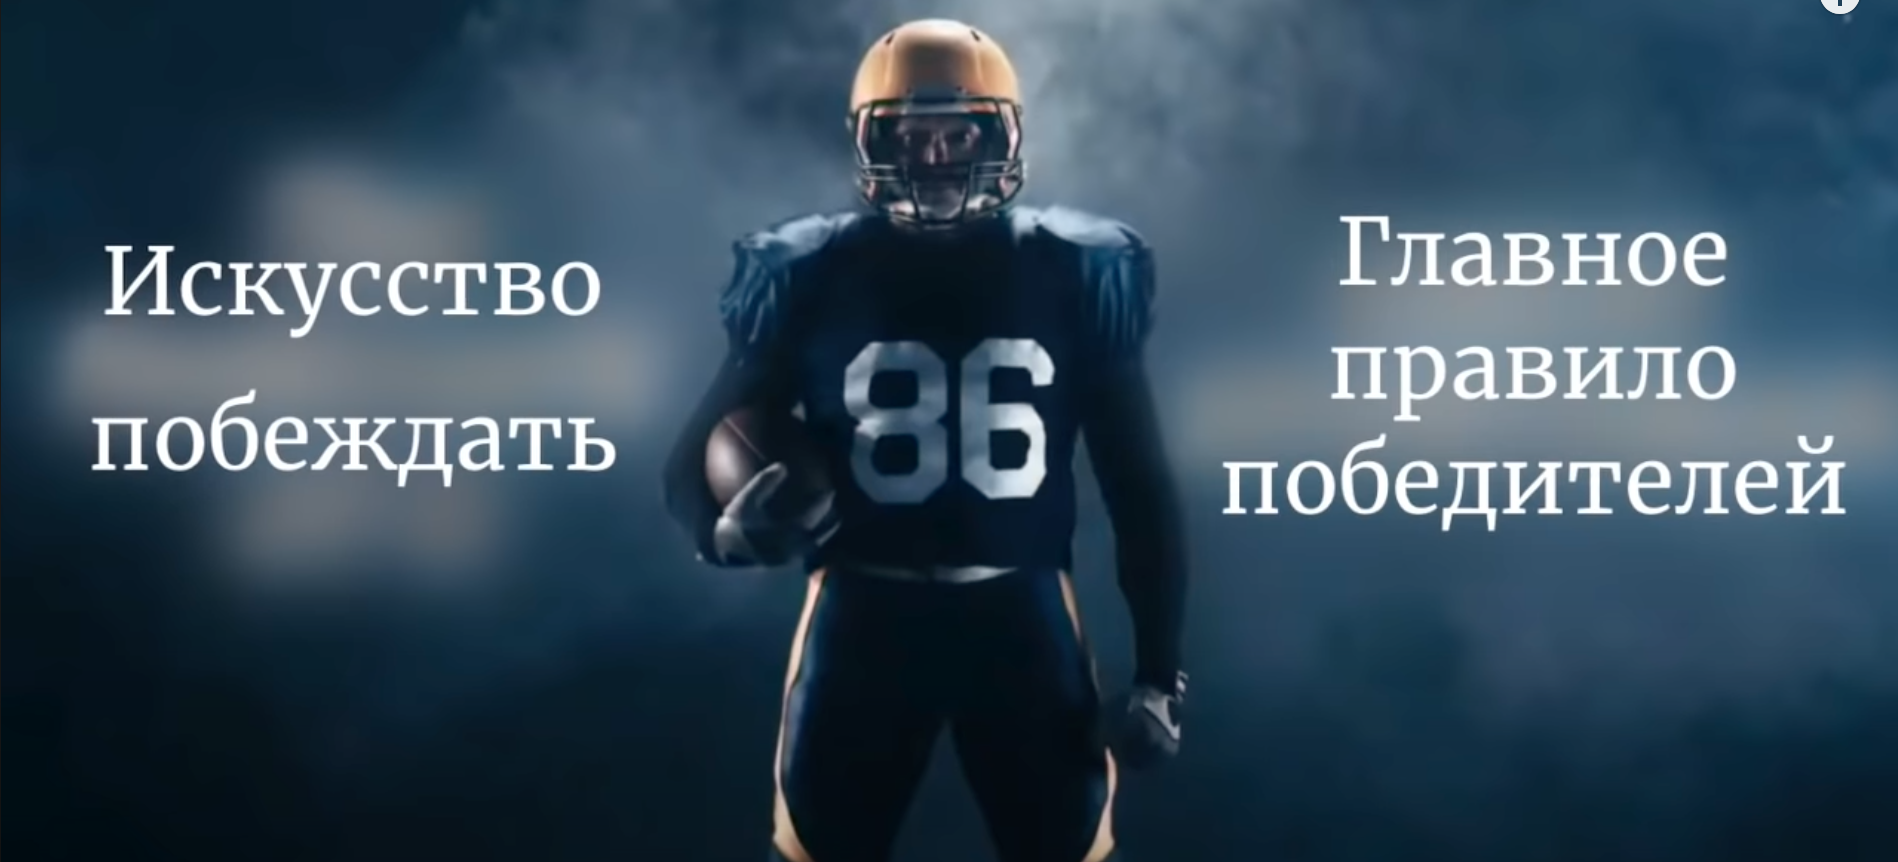
\includegraphics[width=\textwidth]{titleBlur}
\caption{Nice.}
\end{minipage}
\hfill
\begin{minipage}[b]{0.4\textwidth}

\includegraphics[width=\textwidth]{titleBlurBad}
\caption{Not nice.}
\end{minipage}
\end{figure}

\item If the background merges with the translated text,
or blurred English text
adds too much white/black to the background, then
you can add a semi-transparent background to the translated text.
\end{itemize}

\item\emph{Fix the frame when the English text has not yet appeared.}

\begin{itemize}
\item is suitable in the case of a static image on the background. If
there is a beautiful animation on the backdrop~--- blur is preferable.

\item If there is a zoom in the original (dynamic zoom
static image) to add dynamics, then you need
add zoom and when translating.

\end{itemize}
\textit{P.S.} There is a video example of this method in the training materials.

\item \emph{If there is a stem (video without English text).}

In this case, we proceed as follows: download both the original with the text
and the stem. We add them one on top of the other, and mount them. In the end
you can simply disable (make invisible) the track
with English text.

For titles, subtitles, etc. we try, if possible,
choose beautiful effects instead of just the "Text" effect.
\end{itemize}

\subsection{How to download a video}
To download videos from YouTube, you can use the website
\href{https://www.y2mate.com /}{https://www.y2mate.com /} by copying and pasting
the link to the video.

Also, if the video is already open in the browser, you can simply insert "pp" after
the word youtube in the link, and y2mate will open automatically.

For example, https://www.youtube.com/watch?v=Oi7eLmaL1DU need to convert
to https://www.youtube\textbf {pp}.com/watch?v=Oi7eLmaL1DU .

\subsection{Where to mount}
The Isha Foundation mainly uses Final Cut and Adobe Premiere Pro,
but you can use any editor that is convenient for you.

For example, DaVinci Resolve~---
a professional video editor with a free version, which is more than enough for us.

For macOS users, the simplest version of the mounting system is ~---
iMovie, but it has a couple of serious drawbacks.
\begin{itemize}
\item There is no way to conveniently add text over the video.
That is, you will have to do
a picture with a re-image in a separate application and paste it on top.
This disrupts the flow, and you will need to tinker if you have to correct the text.
\item Only two video tracks can be used. This limits more
complex installation, although usually two are enough.
\end{itemize}
Therefore, the advice is~--- download a more professional application, especially since
DaVinci is free =).




\newpage
\section{Training materials}

Mounting is not difficult at all! It will be a little difficult at the beginning, but the basics can
be mastered in a couple of hours. The main thing ~--- is not to be afraid, and ask if something is not clear.

Also, Google~--- is a valuable helper, especially if you Google in English.
For example, queries like
"DaVinci how to add frame hold" ("DaVinci how to fix a video frame")
should help.

Below are real-life examples of installation, you can get acquainted with them!
\begin{itemize}
\item Detailed video is an example of video editing in DaVinci.
An example for a YouTube video, but, in
Instagram, about the same tasks)

DaVinci exmple:~--- \href{https://youtu.be/SAceoBqdAvw}{https://youtu.be/SAceoBqdAvw}
\item A short video on how to fix a frame and add zoom.

DaVinci Frame Freez example:~--- \href{https://youtu.be/caPaZ5syTC8}{https://youtu.be/caPaZ5syTC8}
\item A short tutorial on what to do with old "square" videos.

DaVinci Narrow Video Tutorial:~--- \href{https://youtu.be/FGdErSdSOAI}{https://youtu.be/FGdErSdSOAI}

\item Three two-minute editing videos for Instagram in Premiere Pro.

Premiere short examples:
\begin{itemize}
\item \href{https://youtu.be/AWOsM9fX9RQ}{https://youtu.be/AWOsM9fX9RQ}
\item \href{https://youtu.be/lvRnpvTXHis}{https://youtu.be/lvRnpvTXHis}
\item \href{https://youtu.be/Ontq3mMD9AM}{https://youtu.be/Ontq3mMD9AM}
\end{itemize}
\end{itemize}




\newpage
\section{Test Task (Training video) YouTube}

Task~--- to mount a video and send the result
by a reply message..

You can upload the video directly to Telegram, or post
it on Google Drive and send a link.

\begin{center} \textbf{Video} \end{center}
\href{https://www.youtube.com/watch?v=9sGJUR7stzc}{Original.}
\quad
\href{https://drive.google.com/file/d/1Y6ECjMSvkaUFmNawIePfFvqS2ZnB3SPi/view?usp=sharing }{Audio track.}
\quad
\href{https://www.youtube.com/watch?v=Q3NYDF4JyTg}{Russian-language video for comparison.}

Video title: \textbf{How to live an incredible life}

Translation of the subtitle to 08:10: \textbf{<<Tayir>> in Tamil means yogrt}


\begin{wrapfigure}{r}{0.3\textwidth}
\begin{center}
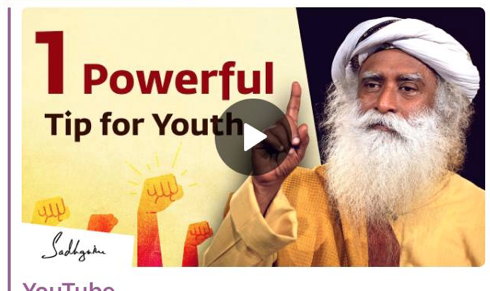
\includegraphics[width=0.28\textwidth]{thumbnail}
\end{center}
\end{wrapfigure}

\emph{P.S.} There is a rather ugly subtitle on the Russian channel, I urge you to improve it =).

\emph{P.P.S.} Thumbnail (picture on the right) is made by a design team, not an editor.


\newpage
\section{Technical points}
\subsection{Installing macOS fonts}\label{fonts}
\begin{enumerate}
\item Download the font, for example, from Google Fonts.
\item Open the application \textbf{"font Book"}.
\begin{center}
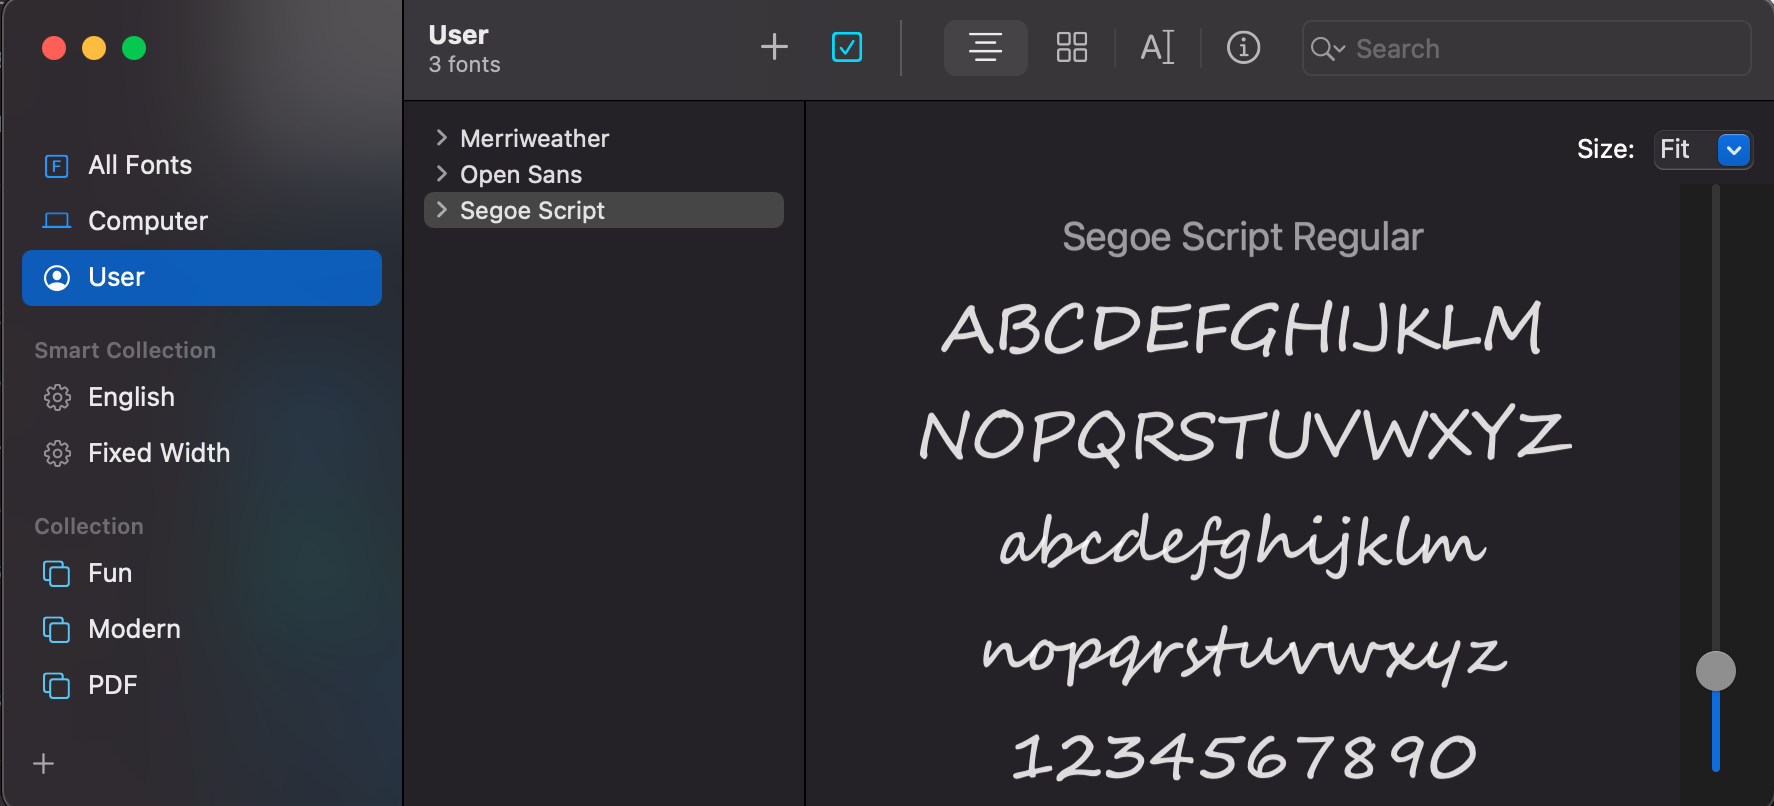
\includegraphics[width=0.9\textwidth]{fontsInstallation/macos0}
\end{center}

\item Click on \textbf{"add fonts"}.
\begin{center}
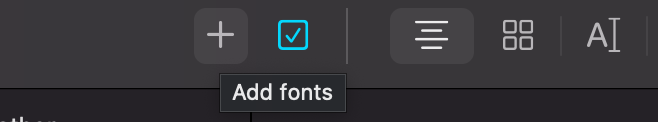
\includegraphics[width=0.5\textwidth]{fontsInstallation/macos1}
\end{center}
\item Select the downloaded file and click on \textbf{"Open"}.
\begin{center}
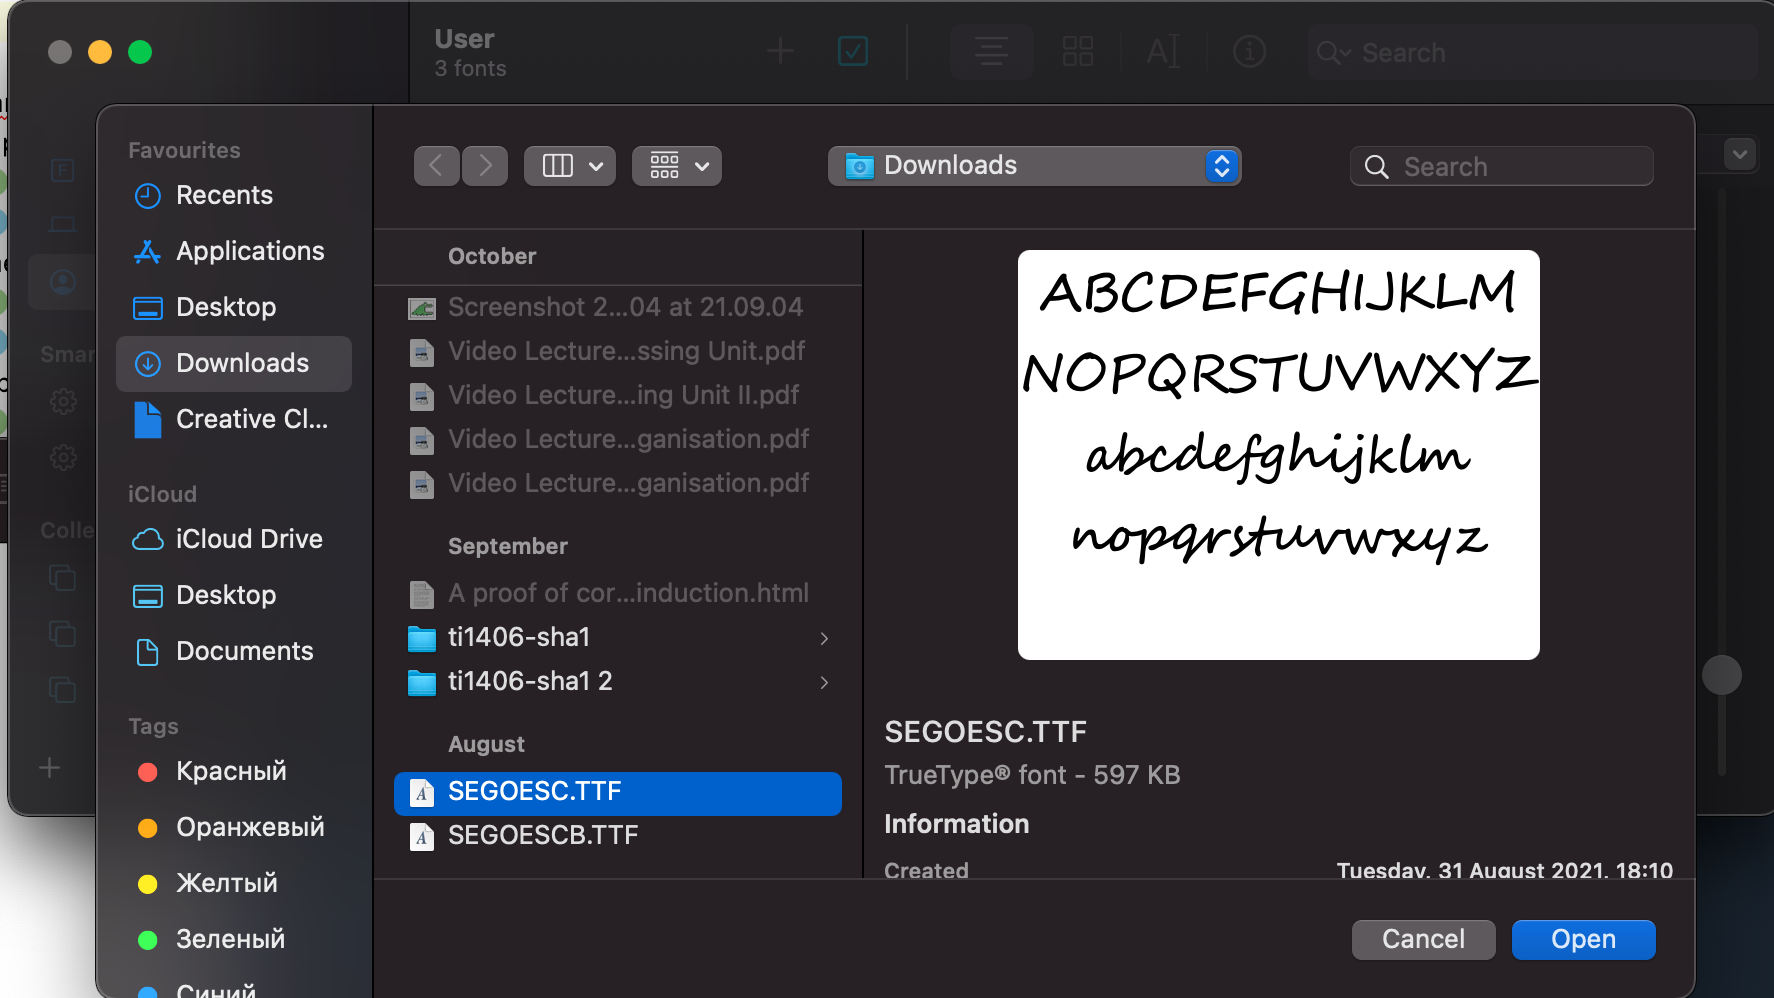
\includegraphics[width=0.9\textwidth]{fontsInstallation/macos2}
\end{center}
\end{enumerate}



\newpage
\thispagestyle{empty}
\tikz[remember picture,overlay]
\node[opacity=0.15,inner sep=0pt] at (current page.center)
{
\includegraphics[width=0.2\paperwidth]{IshaLogo}};
\end{document}

